\begin{figure*}
  \noindent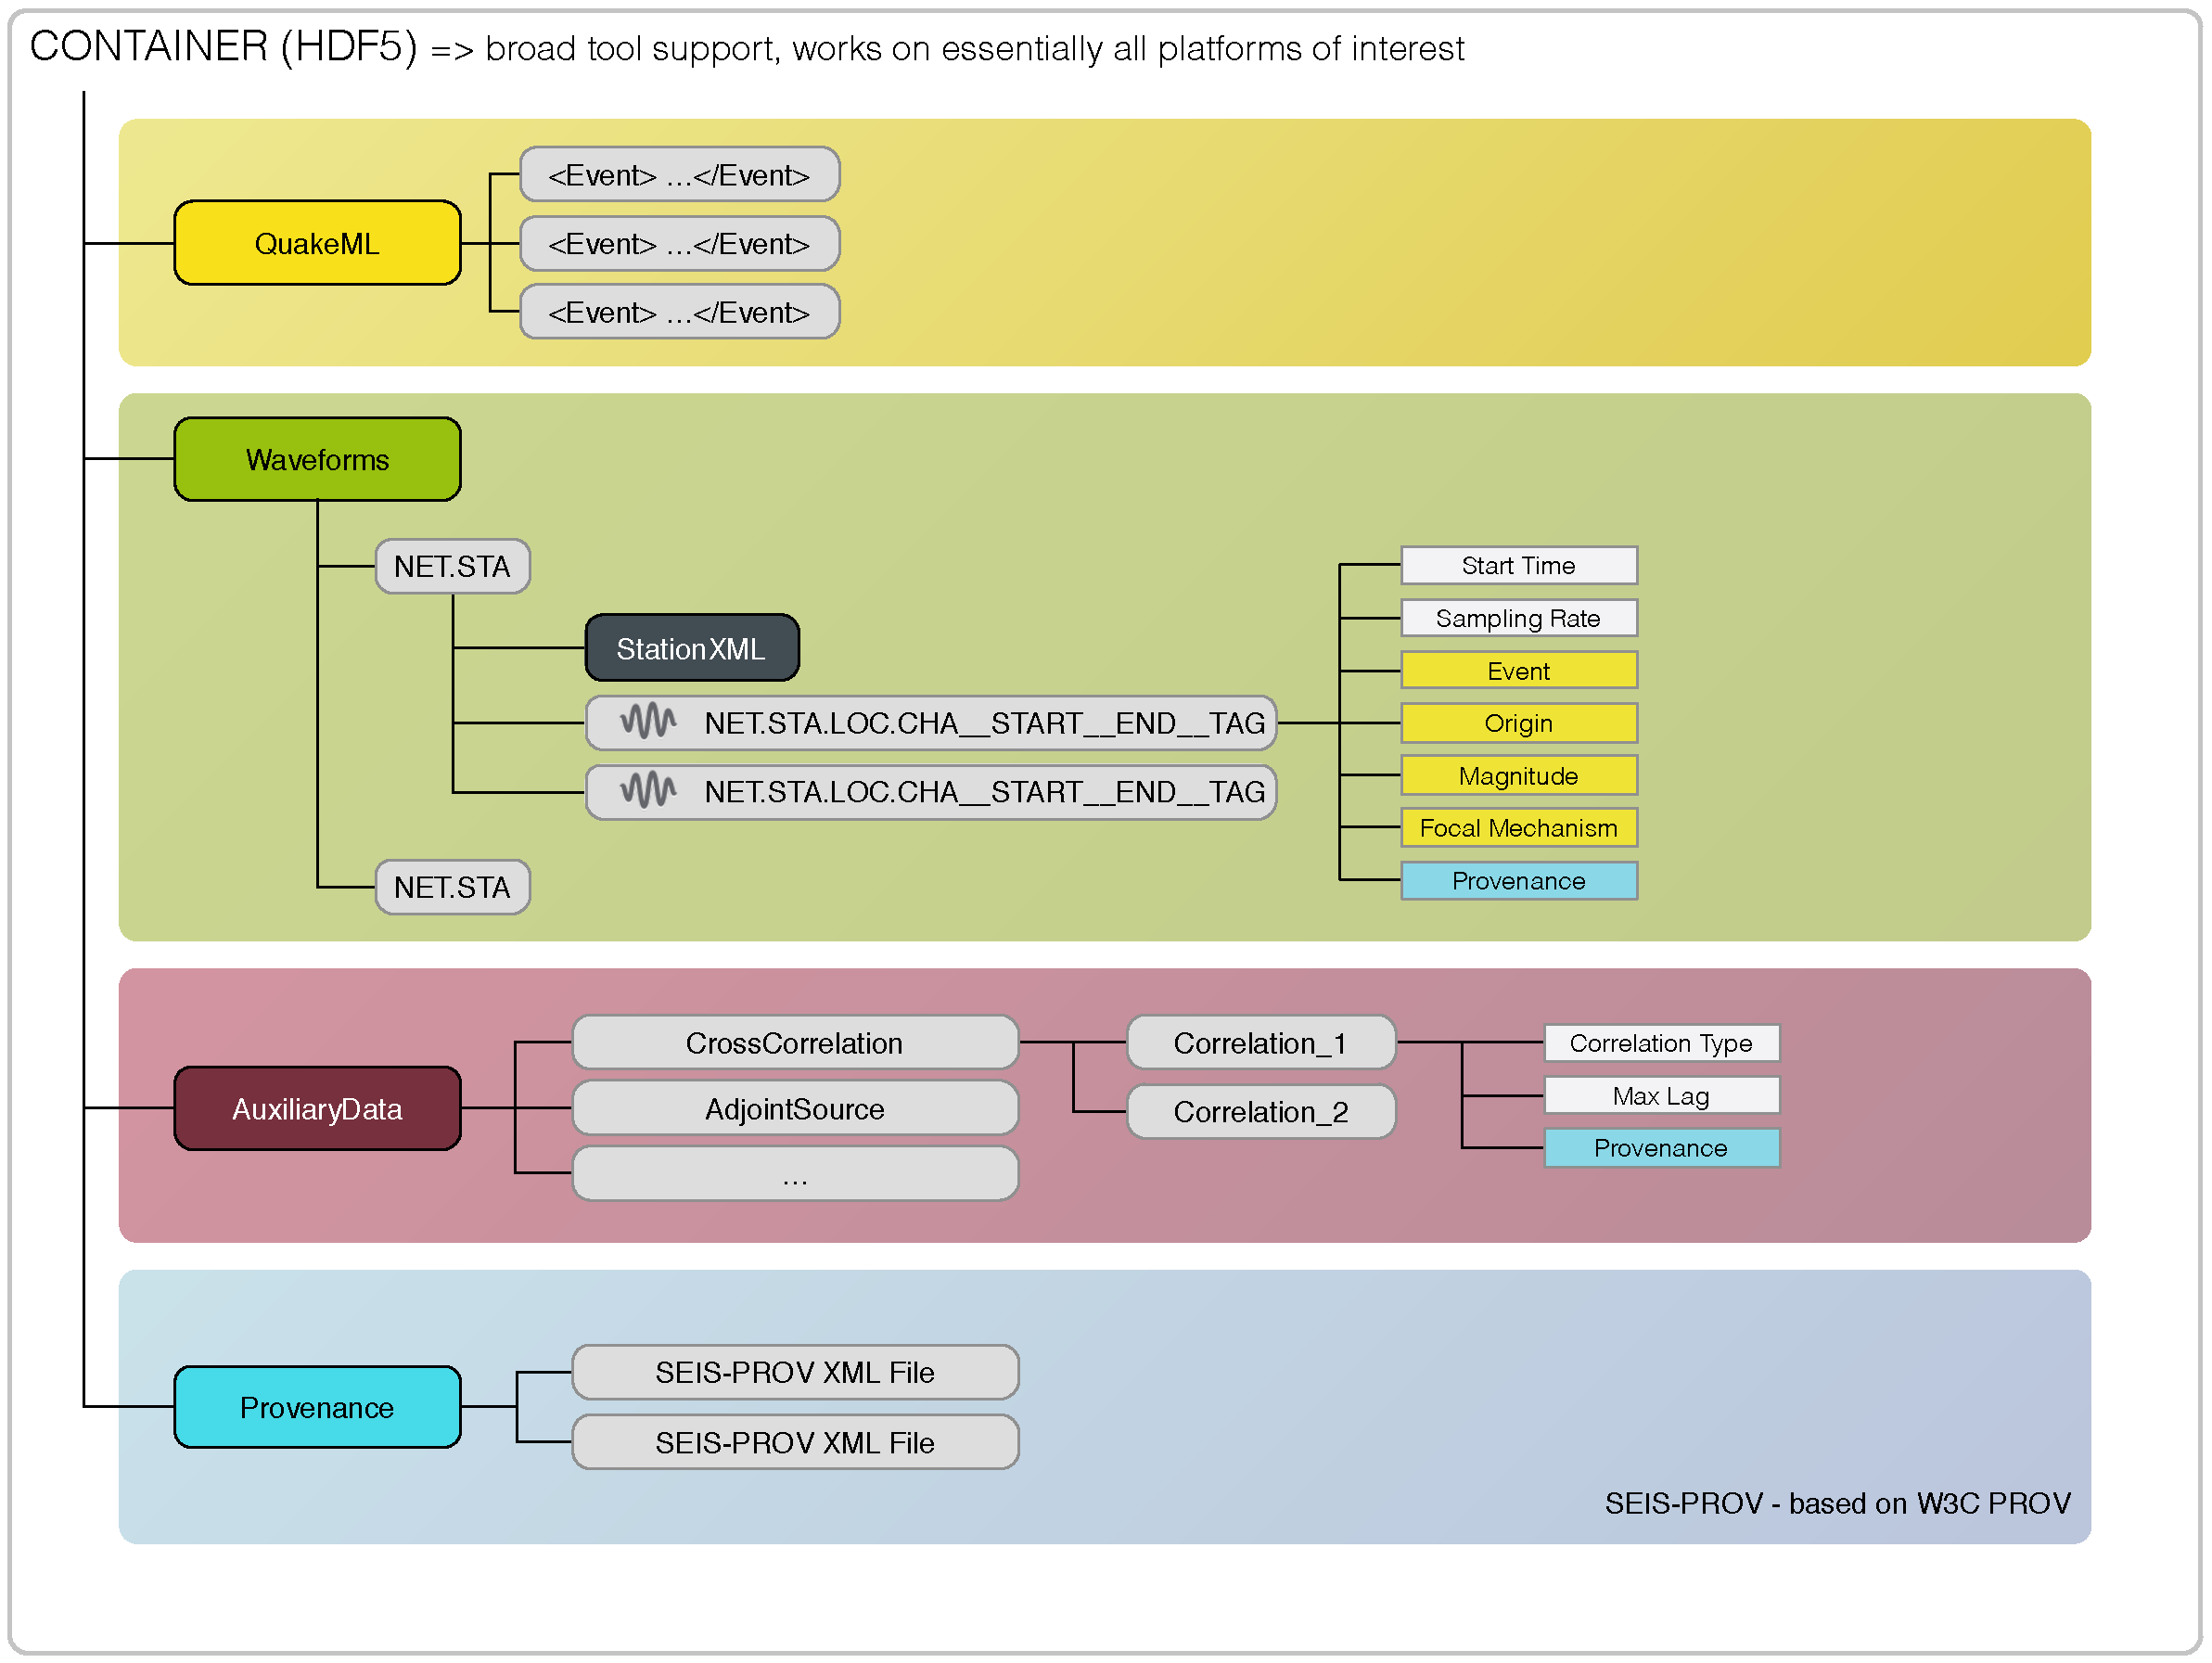
\includegraphics[width=\textwidth]{ch-asdf/figures/ASDF_container}
    \caption[The general structure of an ASDF file]
    {\small{The general structure of an ASDF file in its
        HDF5 container --- it has four distinct parts:
        (1, yellow) Information about an arbitrary number of earthquakes (or
        other seismic events) is stored in a single QuakeML document, the
        most complete earthquake description format currently available.
        (2, green) Seismic waveforms are stored per station together with the
        necessary meta information in the form of an FDSN StationXML
        document.
        (3, red) Anything that cannot be regarded as a seismic waveform is
        hierarchically stored in the auxiliary data section.
        (4, blue) Provenance information is stored as a number of
        SEIS-PROV documents, an extension to W3C PROV.
        Background colors in the attributes (rectangular boxes) denote
        relations to other sections in an ASDF file. Examples of this
        are relations of a waveform to a certain event or a provenance record
        for a piece of auxiliary data.
    }}
    \label{fig:asdf_container}
\end{figure*}


\begin{figure*}
  \noindent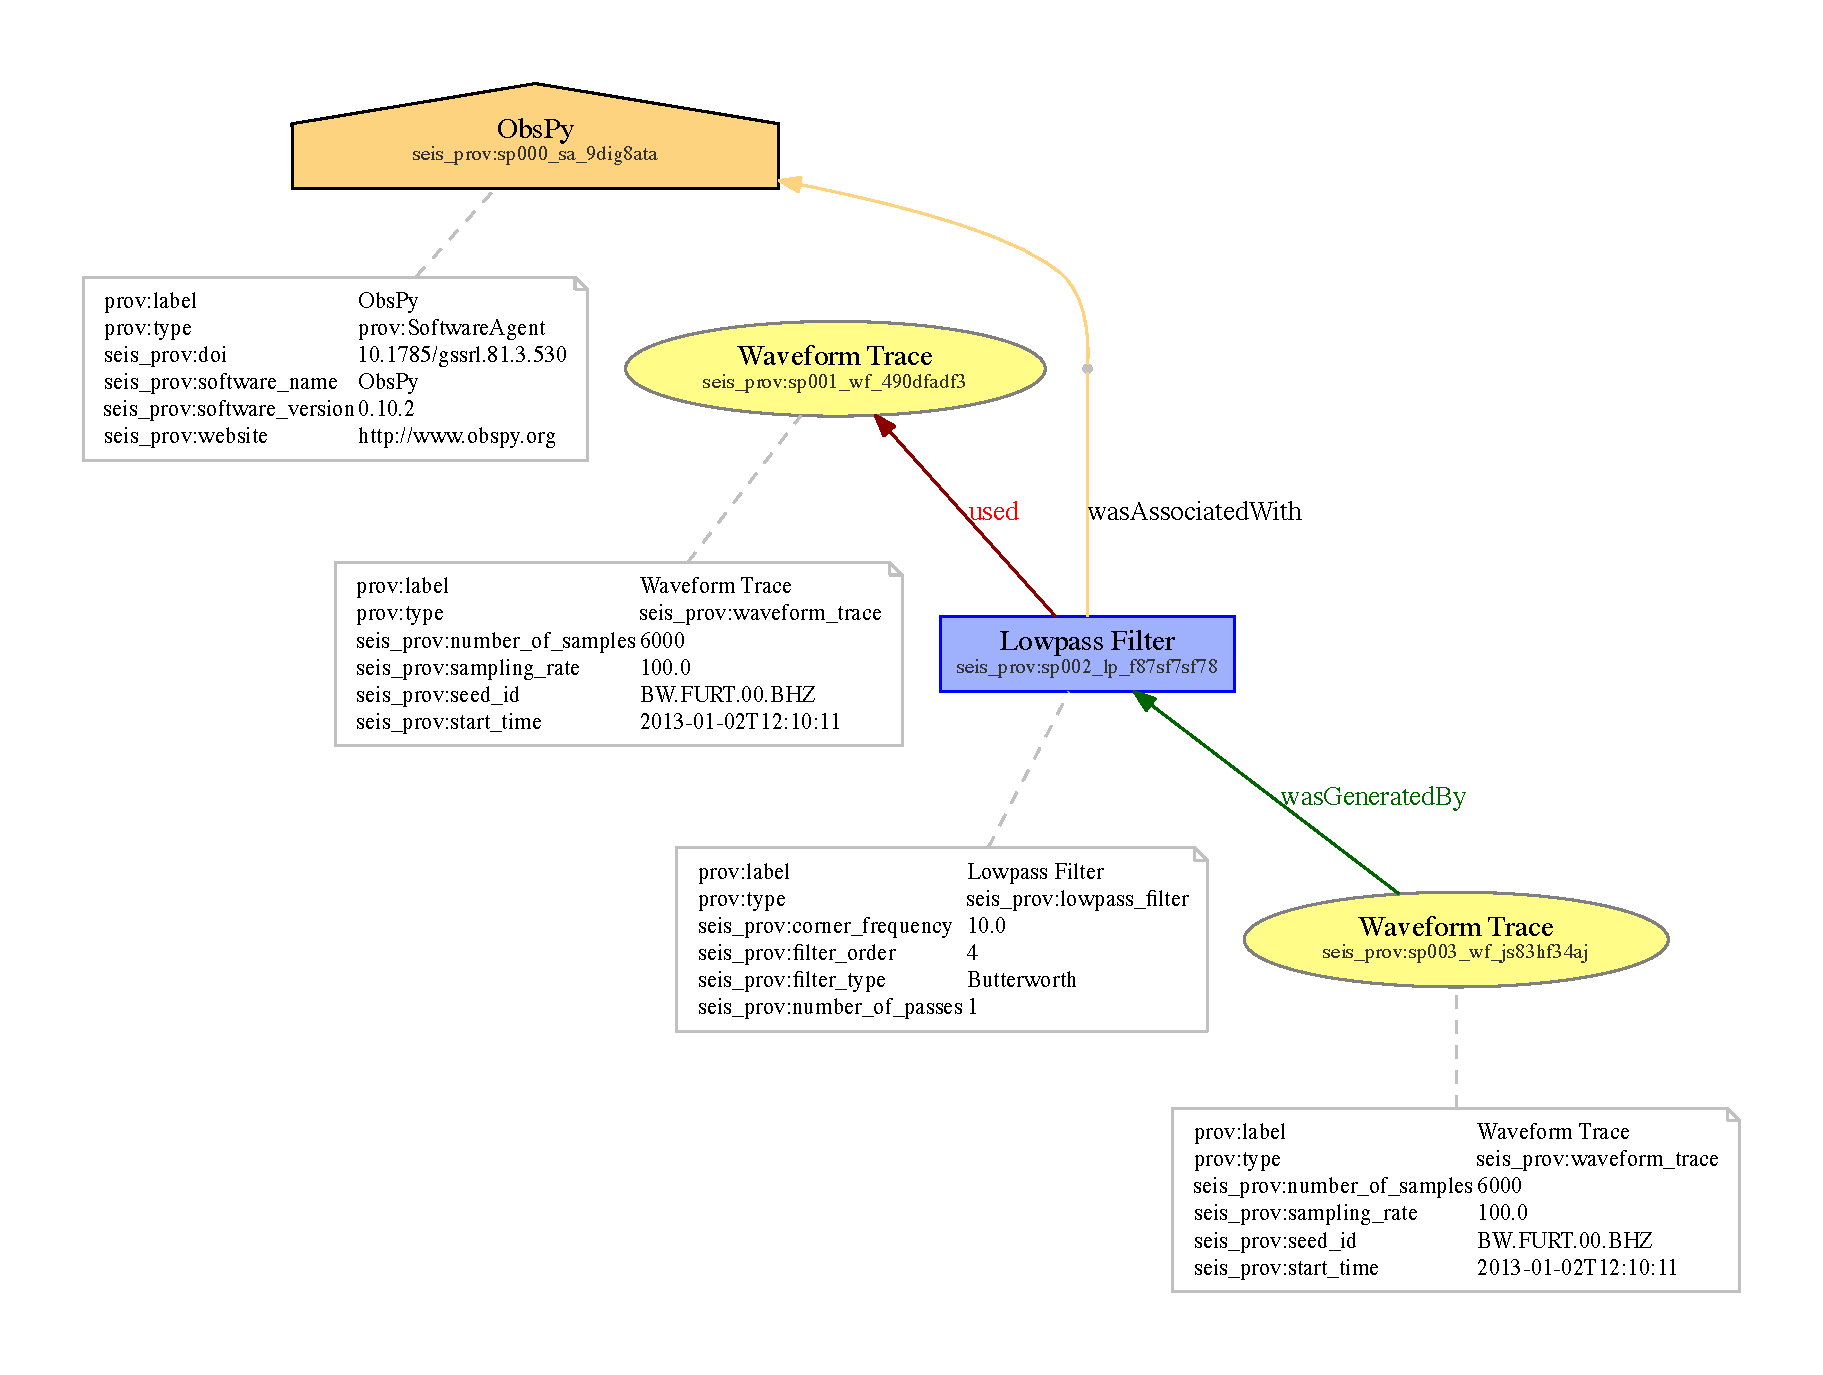
\includegraphics[width=\textwidth]{ch-asdf/figures/simple_provenance}
    \caption[Concepts of storing provenance in ASDF]{\small{
            Simple example to illustrate the key concepts of storing provenance
            information with SEIS-PROV and W3C PROV. It
            describes a single waveform trace that has been lowpass filtered to
            create a filtered waveform trace. The arrows in this graphical
            representation mostly point backwards in the process towards the
            origin of something. The yellow ellipses are called entities, and
            here they represent a waveform trace at two different points in
            time. The blue rectangle is an activity that can use and generate
            entities.  It denotes a lowpass filter and uses the first waveform
            trace to generate a new, filtered waveform trace. The orange house
            shape symbolizes an agent who is responsible for something. In this
            case it stands for the software that performed the filtering
            operation.  Finally, the white rectangles are attributes with more
            details about any node. Please note that this figure shows only one
            possible graphical representation of the underlying data model and
            more or less detailed ones can be employed as appropriate.
    }}
    \label{fig:simple_provenance_example}
\end{figure*}


\begin{figure*}
    \noindent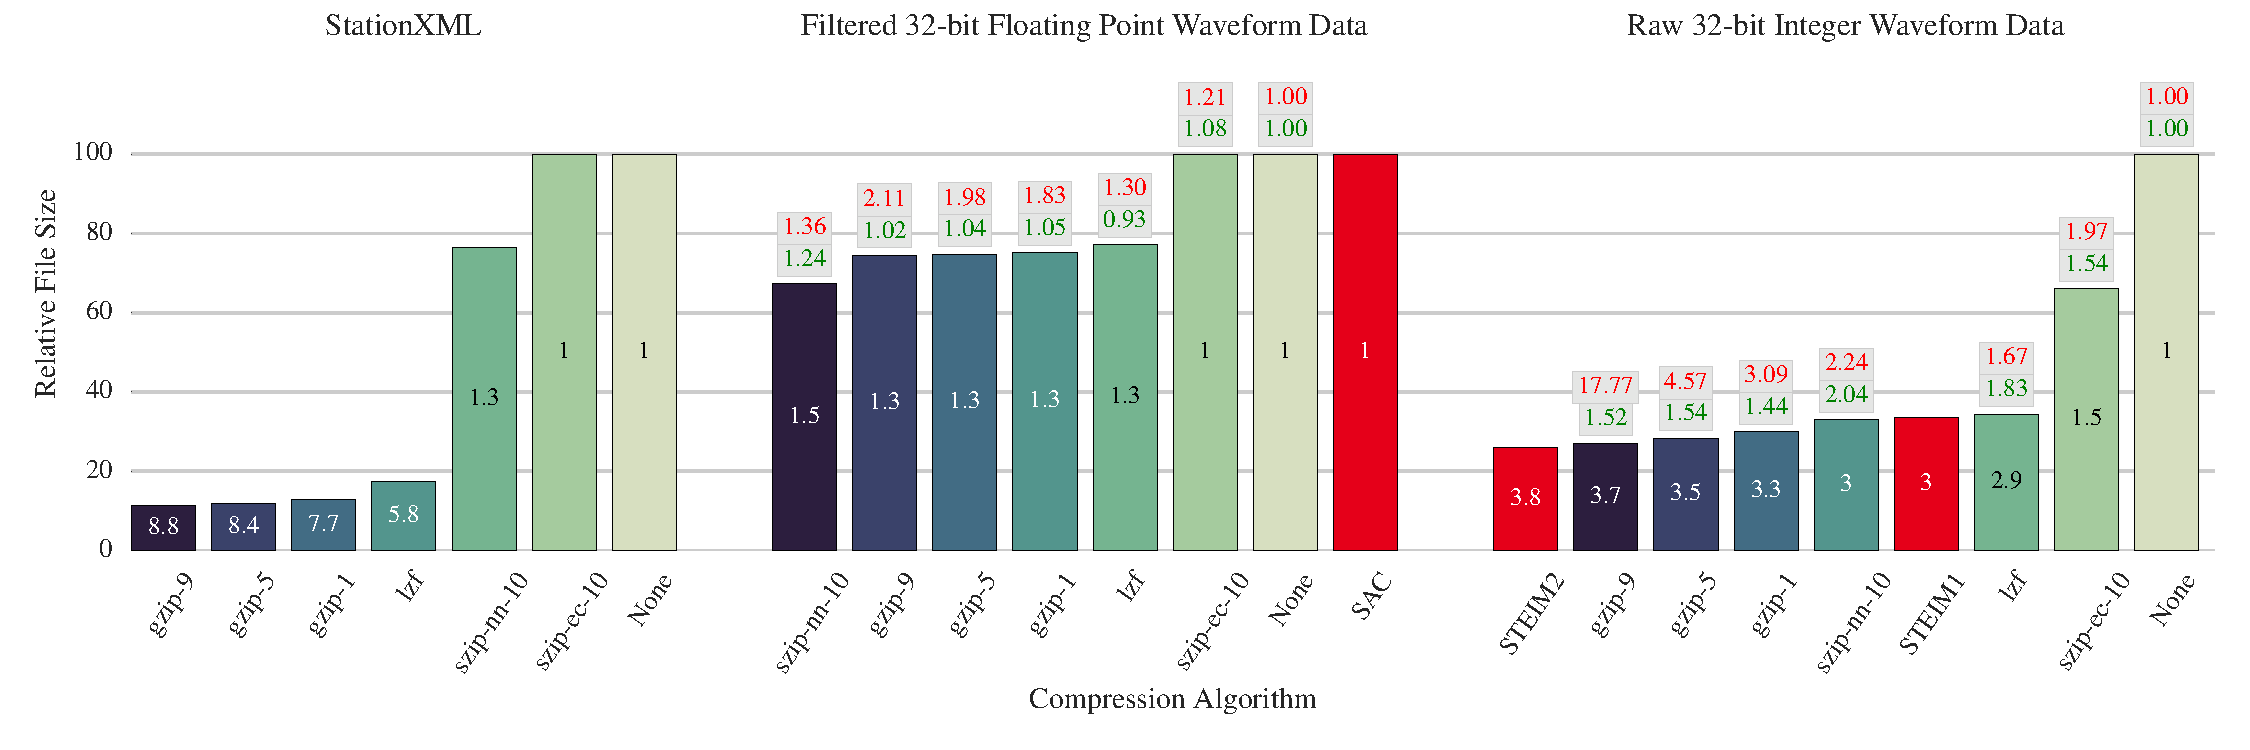
\includegraphics[width=\textwidth]{ch-asdf/figures/ASDF_data_compression}
    \caption[Compression efficiency of the ASDF format]{\small{
        Compression efficiency of the ASDF format using algorithms available in
        HDF5 for a number of typical seismological datasets.  Please keep in
        mind that the efficiency and I/O speed of these algorithms are heavily
        dependent on the actual data and hardware, and thus your mileage may
        vary. The columns represent the file size relative to the uncompressed
        case, the numbers inside are the achieved compression ratios. The small
        boxes above the columns denote the relative writing duration in red and
        the relative reading duration in green compared to the uncompressed
        case. The left plot shows the efficiency for a dataset containing 500
        StationXML documents adding up to 120 MiB. I/O speed differences are
        irrelevant as the cost for parsing and generation of the XML documents
        is constant and dominates the total run time. The middle plot shows the
        compression efficiency for a bandpass filtered waveform dataset stored
        as 32-bit floating point numbers. It consists of 3,466 waveform traces
        taking up 282 MiB on disk. The red bar compares it to the uncompressed
        SAC format. The rightmost plot shows the efficiency for storing 3,346
        raw waveform files stored as 32-bit integers taking up 2,340 MiB. The
        red bars here show the efficiency for the same dataset of the STEIM1
        and STEIM2 special purpose compression algorithms defined for the SEED
        format measured by writing them as MiniSEED files.
    }}
    \label{fig:compression_efficiency}
\end{figure*}
